\section{Cognitive Architectures}
\label{sec:cogarch}
Cognitive architectures are architectures that base themselves on some model of
human cognition. There are several competing models of cognition, and one of
the most recent and well-supported is the Global Workspace Theory.

One area that haven't been as well explored in relation to RTSes in general and
StarCraft in particular, is cognitive architectures. Arrabales et al put forth
that this is perhaps because of poor understanding within the field of classical
AI of research into cognition\cite{arrabales2009gamechars}.

\subsection{Global Workspace Theory}

\begin{figure}[h!tb]
\centering
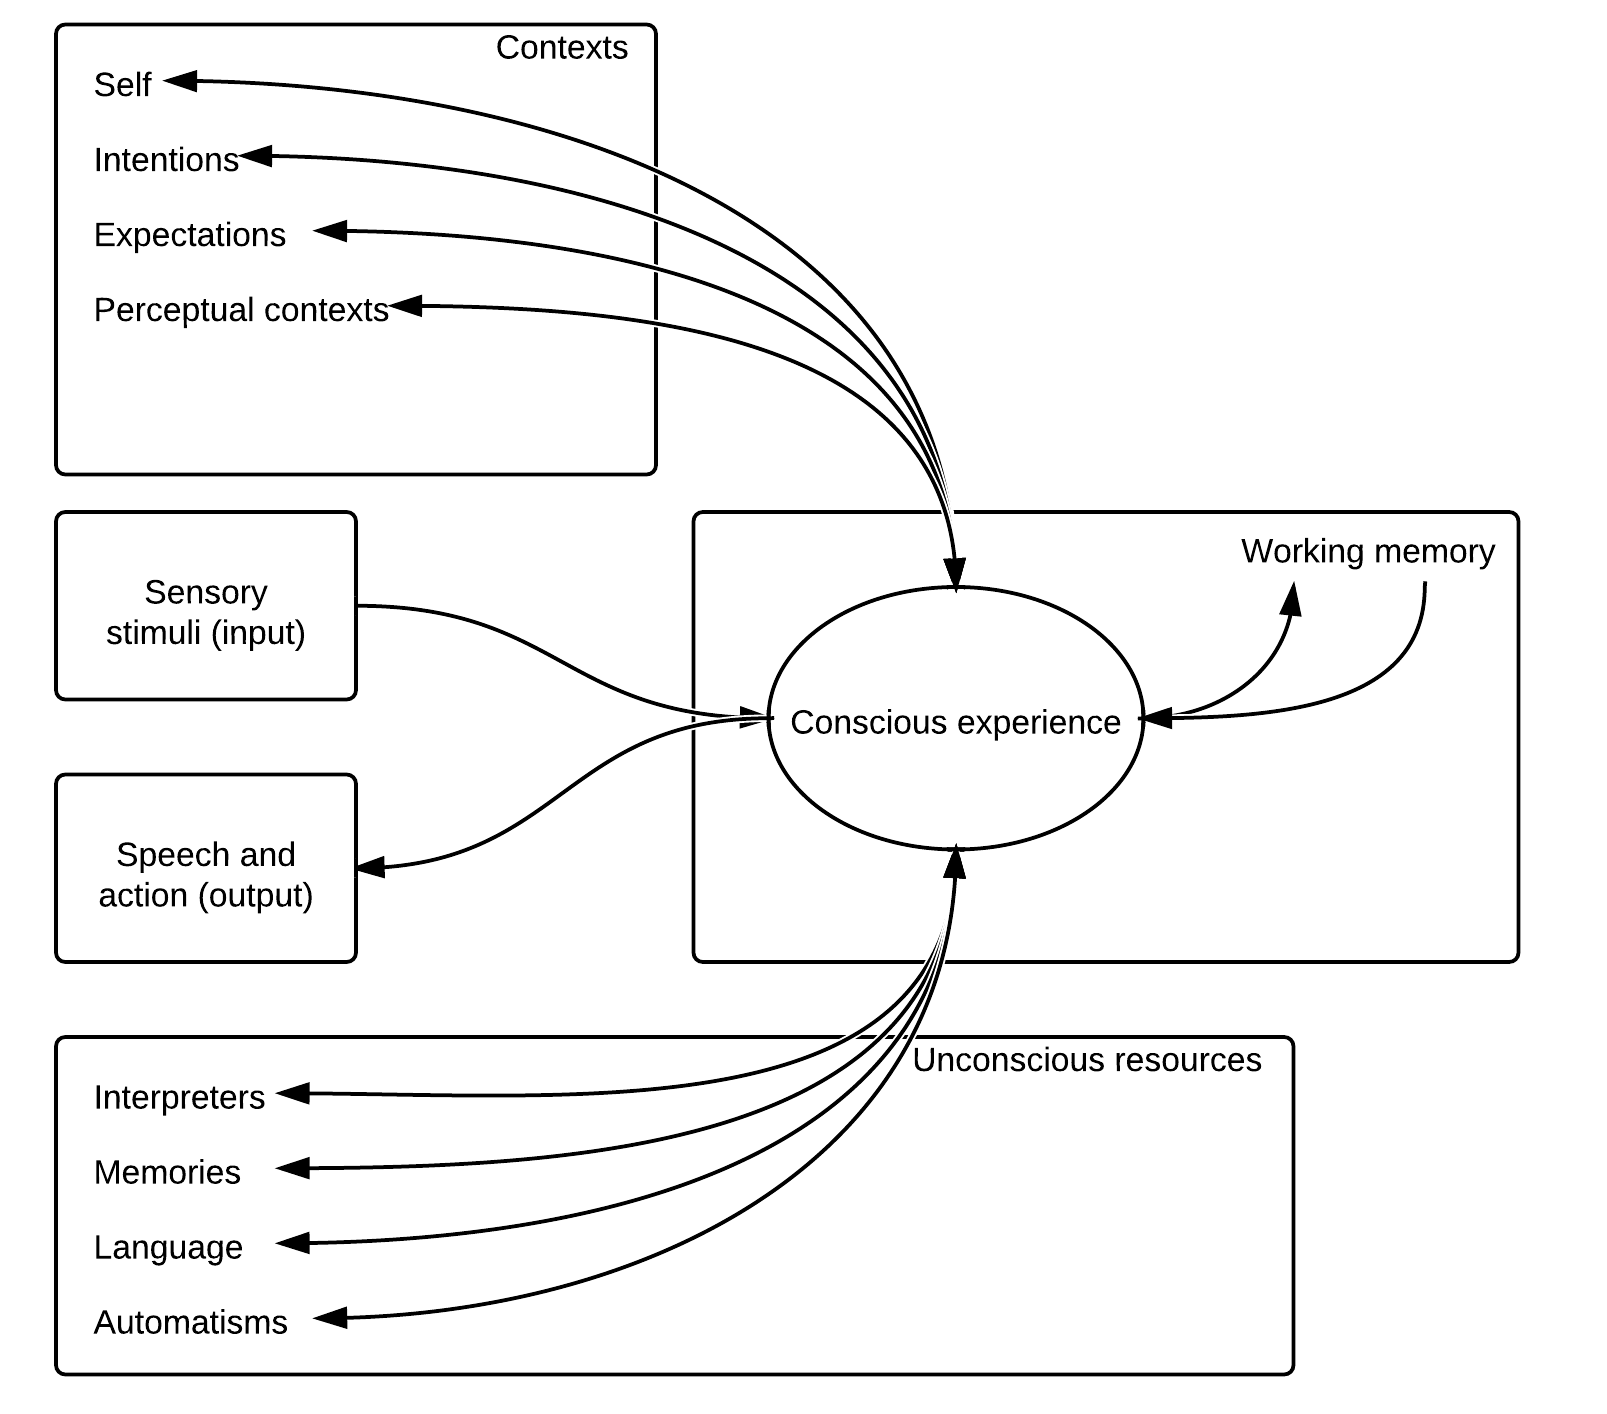
\includegraphics[scale=1.0]{graphics/globalworkspace.png}
\caption{A schematic of the Global Workspace theory\cite{baars2005gwt}}
\label{fig:gwt}
\end{figure}

Global Workspace Theory is a model of cognition that is very well supported by
experimental data, and is one of the most widely accepted
models.\cite{dehaene2001towards} It has been used to implement processes that
imitate human decision making (for example for solving the problem of assigning
people to jobs in the US Navy).\cite{baars2005gwt}\cite{franklin2003interacting}

It is based around an understanding of the brain as a set of many independently
processing modules, working together by utilizing a shared workspace (hence the
``global workspace''). Every ``cognitive cycle'' all the
processes compete for attention, and a single one gets the
proverbial spotlight shone upon it.\cite{baars2005gwt}

There have been several implementations of GWT for different domains and
approaches, for example the LIDA (``Learning IDA'')
model\cite{franklin2007lida}, or the CERA-CRANIUM
architecture\cite{arrabales2009ceracranium}.

See figure \ref{fig:gwt} for an overview of the theory.

\subsection{Cognitive Models in Game AIs}
There have been several more or less successful attempts at implementing models
of cognition into game-playing agents. One of the more recent ones is
CERA-CRANIUM. One of the reasons for using computer games for experiments with regards to
high-level artificial intelligence is that the characteristics of computer
games lend themselves to this, by eliminating noise and uncertainty, and
providing a more or less realistic simulated environment.

\subsection{The LIDA Model}
The LIDA model is a cognitive model based on the GWT.